\documentclass[fleqn]{jbook}
\usepackage{physpub}

\begin{document}

\begin{question}{$B@l96(B $BLdBj(B3}{}


$B<'>l(B$H$$BCf$G$NBg$-$5(B$J\;(=1/2,1,3/2,\cdots)$$B$N%9%T%s$N%(%M%k%.!<(B
$B8GM-CM(B$\varepsilon_m$$B$O!"(B
%
\[ \varepsilon_m = g\mu_BHm, \hspace{10mm}(m=-J,-J+1,\cdots,J-1,J) \]
%
$B$GM?$($i$l$k!#$3$3$G!"(B$m$$B$O<'5$NL;R?t!"(B$g$$B$O(B$g$$B0x;R!"(B$\mu_B$$B$O%\!<%"(B
$B<';R$G$"$k!#$3$N$h$&$J%9%T%s$rC10LBN@QCf$K(B$n$$B8D4^$_!"29EY(B$T$$B$NG.J?9U(B
$B>uBV$K$"$k7O$K$D$$$F!"0J2<$NLd$KEz$($h!#$?$@$7!"%\%k%D%^%sDj?t$r(B$k$
$B$H$7!"%9%T%s$N4V$NAj8_:nMQ$O9M$($J$$!#(B


\begin{subquestions}
\SubQuestion
  $B$3$N7O$NC10LBN@Q$"$?$j$NJ,G[4X?t$O<!<0$GM?$($i$l$k$3$H$r<($;!#(B
%
  \[ Z = \left(\frac{\sinh[(2J+1)x/2J]}{\sinh(x/2J)}\right)^n,%
     \hspace{1cm}x=\frac{g\mu_BJH}{kT} \]
%

\SubQuestion
  $B$3$N7O$NC10LBN@Q$"$?$j$NHfG.(B$C$$B$r<!<0$GDj5A$5$l$k%V%j%k%"%s4X?t(B
  $B_J(x)$$B$NF34X?t$rMQ$$$FI=$;!#(B
%
  \[ B_J(x) = \frac{2J+1}{2J}\coth\left(\frac{2J+1}{2J}x\right)
             -\frac{1}{2J}\coth\left(\frac{x}{2J}\right) \]
%

\SubQuestion
  $B29EY$,(B(a)$B9b$$>l9g(B($x\ll 1)$$B$H(B(b)$BDc$$>l9g(B($x\gg J)$$B$K$D$$$F!"(B
  $BHfG.(B$C$$B$N6a;w7A$r5a$a$h!#(B


\SubQuestion
  $BA0Ld$N7k2L$K4p$E$-!"(B$J=1/2$$B$KBP$7$F!"HfG.(B$C$$B$N29EY0MB8@-$N35N,$r(B
  $B?^<($7!"$3$N$h$&$J29EY0MB8@-$H$J$kJ*M}E*M}M3$r=R$Y$h!#$J$*!"?^$O(B
  $B=D<4$r(B$C/nk$$B!"2#<4$r(B$kT/g\mu_BJH$$B$H$;$h!#(B


\SubQuestion
  $B8EE5%9%T%s$N6K8B(B($B@Q(B$g\mu_BJ$$B$,0lDj$N$^$^(B
  $J\rightarrow \infty,\;g\mu_B\rightarrow 0$$B$H$7$?>l9g(B)
  $B$K$*$1$kHfG.(B$C$$B$r5a$a$h!#$5$i$K!"$=$N29EY0MB8@-$N35N,$r<($;!#(B
  $B$J$*!"?^$OA0LdF1MM!"=D<4$r(B$C/nk$$B!"2#<4$r(B$kT/g\mu_BJH$$B$H$;$h!#(B

--------------------------------------------------------------------------------------------------------------\\
($B;29M(B)$B%V%j%k%"%s4X?t(B
%


\begin{minipage}{90mm}
  $B1&?^$K(B$J=1/2,1,2,4,8$$B$KBP$9$k%V%j%k%"%s4X?t$r<($9!#(B\\
  $B6a;w<0(B($B>ZL@$J$7$KMQ$$$F$h$$(B)
  \begin{eqnarray*}
    B_J(x) &\approx& \left\{\begin{array}{ll}%
      \ds \frac{J+1}{3J}x &%
      (x\ll 1) \\[2mm]
      \ds 1-\frac{1}{J}\exp\left(-\frac{x}{J}\right) &%
      (x\gg J)%
    \end{array}\right.\\
%
    \coth(x) &\approx& \left\{\begin{array}{ll}%
      \ds \frac{1}{x}+\frac{x}{3}\quad\quad\quad\quad\;\;&
      (x\ll 1)\\[2mm]
      \ds 1+2e^{-2x} &
      (x\gg 1)%
    \end{array}\right.
  \end{eqnarray*}
\end{minipage}
\begin{minipage}{70mm}
  \begin{center}
    \mbox{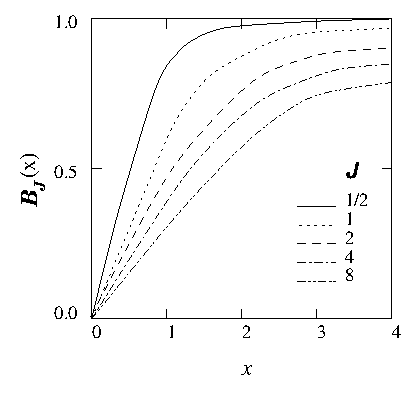
\includegraphics[clip]{1994phy3-1.eps}}
  \end{center}
\end{minipage}


\end{subquestions}
\end{question}
\begin{answer}{$B@l96(B $BLdBj(B3}{}

\begin{subanswers}
\SubAnswer
  $B3F%9%T%s4V$NAj8_:nMQ$O9M$($J$$$N$G!"A47O$NJ,G[4X?t$O(B1$B$D$N%9%T%s$N(B
  $B$NJ,G[4X?t$N(B $n$ $B>h$G$"$k!#(B
%
  \begin{eqnarray*}
    Z &=&   \left( \sum_{m=-J}^{J} \exp\left(%
            \frac{g\mu_B H}{kT}m\right) \right)^{n}%
       =    \left( \sum_{m=-J}^{J} \exp\left(%
            \frac{x}{J}m\right) \right)^{n}%
       =  \left( \frac{e^{-Jx/J}(e^{(2J+1)x/J}-1)}%
                 {e^{x/J}-1} \right)^{n} \\
      &=&  \left( \frac{e^{(2J+1)x/2J}-e^{-(2J+1)x/2J})}%
                 {e^{x/2J}-e^{-x/2J}} \right)^{n}%
       =   \left( \frac{\sinh[(2J+1)x/2J]}{\sinh(x/2J)}\right)^{n}
  \end{eqnarray*}



\SubAnswer
  $BJ?6Q%(%M%k%.!<(B$U$$B$O(B
%
  \begin{eqnarray*}
    U &=& \frac{\sum{\varepsilon e^{-\beta \varepsilon}}}%
          {\sum e^{-\beta \varepsilon}}%
       = - \Partial{}{\beta} \ln{Z}%
       = -ng \mu_B JH\Partial{}{x} \left(%
            \ln{(\sinh{(2J+1)x/2J})}-\ln{(\sinh{x/2J})} \right) \\
      &=& -ng \mu_B JH \left(%
           \frac{2J+1}{2J}\coth{\frac{2J+1}{2J}x}%
          -\frac{1}{2J}\coth{\frac{1}{2J}x} \right)%
       =  -ng \mu_B JH B_J(x) \\[2mm]
    \Yueni C &=& \Deriver{U}{T}%
       =  \Deriver{x}{T} \Deriver{U}{x}%
       =  \frac{n(g \mu_B JH)^2}{kT^2}B_J'(x)
       =  nkx^2 B_J'(x)
  \end{eqnarray*}


\SubAnswer
  \[ T \rightarrow \makebox[10mm]{\bf\rm large},\quad x \ll 1 \qquad%
     C \simeq nkx^2 \frac{J+1}{3J}%
       =      \frac{J+1}{3J} nkx^2 \]
  \[ T \rightarrow \makebox[10mm]{\bf\rm small},\quad x \gg J \qquad%
     C \simeq \frac{nkx^2}{J^2}\exp{\left(-\frac{x}{J}\right)} \]
%

\SubAnswer
  \parbox[t]{88mm}{
  $J=1/2$ $B$J$N$G(B
%
  \[ x\ll 1 \qquad \frac{C}{nk} \simeq x^2  \]
  \[ x\gg J \qquad \frac{C}{nk} \simeq 4x^2 \exp(-2x) \]
%
  $T \rightarrow$$BBg$G$O!"%9%T%s$N8~$-$OA4$/%i%s%@%`$H$J$j!"(B\\
  $\Mean{E} \rightarrow 0$$B!"$h$C$F(B $C \rightarrow 0$$B!#(B\\
  $T \rightarrow$$B>.$G$O!"%(%M%k%.!<$r:G>.$K$9$k$?$a!"%9%T%s$,$9$Y$F(B
  $m=+J$$B$K$=$m$C$F$7$^$&$N$G(B $C \rightarrow 0$$B!#(B
  }\parbox[t]{75mm}{\vspace*{-5mm}
  \begin{center}
    \mbox{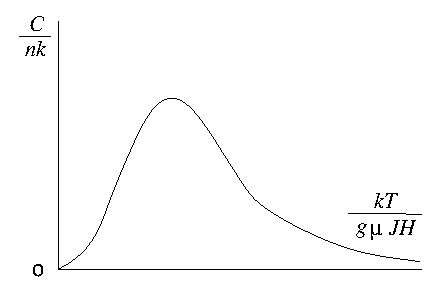
\includegraphics[clip]{1994phy3-2.eps}}
  \end{center}}


\SubAnswer
  $x,\,g \mu_B J$$B$rM-8B$N0lDjCM$K$7$?$^$^!"(B$J \rightarrow \infty$$B$H$9$k!#(B
%
\begin{align*}
	\lim_{J\rightarrow\infty}B_J(x)
	& = \lim_{J\rightarrow\infty}
		\biggl(\frac{2J+1}{2J}\coth\frac{2J+1}{2J}x
			-\frac{1}{2J}\coth\frac{1}{2J}x\biggr) \\
	& =  \coth x
		-\lim_{J\rightarrow\infty}\frac{1}{2J}
			\biggl(\frac{2J}{x}+\frac{1}{3}\frac{x}{2J}\biggr) \\
	& =  \coth x-\frac{1}{x}
\end{align*}
  \[ \lim_{J\to\infty} U%
      = -ng \mu_B JH \lim_{J\to\infty}%
         \left( \frac{2J+1}{2J}\coth{\frac{2J+1}{2J}x}%
              - \frac{1}{2J}\coth{\frac{1}{2J}x} \right)%
      =  -ng \mu_B JH \left( \coth x -\frac{1}{x} \right) \]
%
$B=>$C$F!"HfG.$O(B
\begin{align*}
	C & = nkx^2\Deriver{}{x}\biggl(\coth x-\frac{1}{x}\biggr) \\
	& = nk(1-x^2\cosech^2x)
\end{align*}
$B$H$J$k!#$h$C$F!"(B


  \parbox[t]{88mm}{
  \begin{eqnarray*}
     \hspace{-10mm}x\ll 1 \qquad%
     U &=& -ng \mu_B JH \left( \frac{x}{3} \right) \\
     \Yueni%
     C &=& \Deriver{U}{T} =\frac{n(g\mu_BJH)^2}{3kT^2}%
        = \frac{nkx^2}{3} \\
     \hspace{-10mm}x\gg 1 \qquad%
     U &=& -ng \mu_B JH \left( 1+2e^{-2x}-\frac{1}{x} \right) \\
     \Yueni%
     C &=& \Deriver{U}{T}%
       = \frac{n(g\mu_BJH)^2}{kT^2}\left(\frac{1}{x^2}-4e^{-2x}\right)\\
       &=& nk(1-4x^2e^{-2x})
  \end{eqnarray*}
%
  }\parbox[t]{75mm}{
  \begin{center}
    \mbox{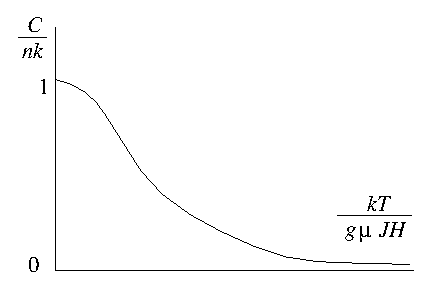
\includegraphics[clip]{1994phy3-3.eps}}
  \end{center}}

\end{subanswers}
\end{answer}


\end{document}
